% =====================================================================
% ch03a.tex —— 第 3 节前半（PDF p.9–13，原书 p.8–12）
% 译者：tr03a；体例见 work/style_guide.md
% 底本：Xi Yin, Aspects of 2D CFTs, PoS(TASI2017)003
% =====================================================================

\section{Virasoro 共形块}\label{sec:3}

\begin{keytakeaways}
  \item 核心物理图像：球面四点函数按 OPE 通道 $12\to 34$ 分解，每个共形块收集中间原初场及其全部 Virasoro 后代的贡献。
  \item 使用的数学工具：共形 Ward 恒等式、Virasoro 后代 Gram 矩阵之逆 $G^{NM}(c,h)$、Kac 行列式的零点、超几何函数。
  \item 本节结论：共形块在 $|z|<1$ 内收敛；它在 $h$ 平面与 $c$ 平面的极点位置由 Kac 行列式给出，留数由融合多项式与低一阶共形块表示，由此得到递推表示。
\end{keytakeaways}

我们首先考虑球面上原初场 $\phi_i(z_i,\bar z_i)$ 的四点函数，其中 $i=1,2,3,4$。如前所见，若把 $\phi_i$ 两两的算符乘积展开（OPE）写成对一整组原初场的 Virasoro 后代求和，四点函数便由共形 Ward 恒等式用结构常数 $C_{12k},C_{34k}$ 确定。下面具体做这个计算。利用黎曼球的共形 Killing 群 $PSL(2,\mathbb{C})$，可以把四个算符放在
\begin{equation}\label{eq:3-1}
  z_1=0,\qquad z_2=z,\qquad z_3=1,\qquad z_4=\infty .
\end{equation}

为使关联函数有限且定义良好，在 $z_4\to\infty$ 极限下对 $\phi_4(z_4,\bar z_4)$ 作重标度，定义为
\begin{equation}\label{eq:3-2}
  \phi_4'(\infty)=\lim_{z_4,\bar z_4\to\infty} z_4^{2h_4}\bar z_4^{2\tilde h_4}\phi_4(z_4,\bar z_4).
\end{equation}

% [Tutor Note: (3.2) 中 $\phi_4'(\infty)$ 的撇号表示重标度后的算符，不是对 $z$ 求导。指数取 $2h_4$ 而非 $h_4$，来自反演 $z\to 1/z$ 的 Jacobian 因子 $(dz'/dz)^{-h_4}=(-z^{-2})^{-h_4}\sim z^{2h_4}$；再乘上反全纯部分 $\bar z_4^{2\tilde h_4}$，极限才有限。]

现在可以计算关联函数
\begin{equation}\label{eq:3-3}
  \langle\phi_1(0)\phi_2(z,\bar z)\phi_3(1)\phi_4'(\infty)\rangle .
\end{equation}

在径向量子化下，可把 $\phi_1(0)$ 与 $\phi_4'(\infty)$ 分别看作 ket 与 bra，四点函数于是等价地写成
\begin{equation}\label{eq:3-4}
  \langle\phi_4|\phi_3(1)\phi_2(z,\bar z)|\phi_1\rangle .
\end{equation}

\begin{figure}[htbp]
  \centering
  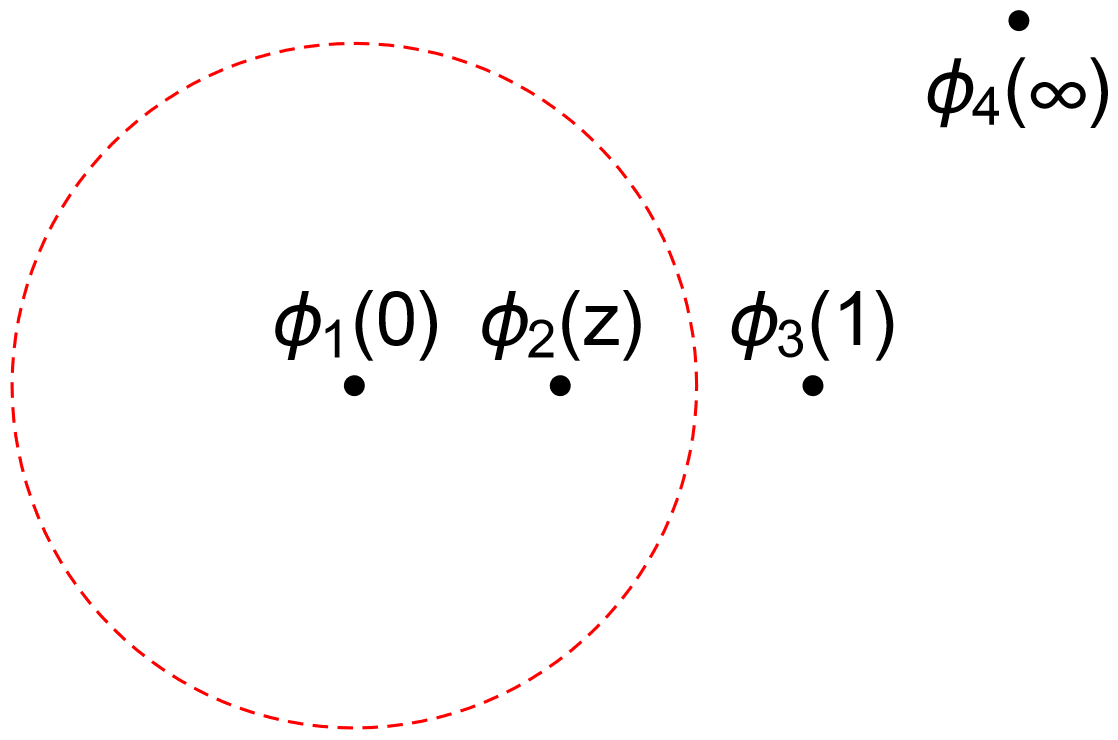
\includegraphics[width=0.85\textwidth]{figures/fig05.png}
  \caption{在四点函数中插入一组完备的态基（红色虚线圈）。（原文 p.8，图 5）}
  \label{fig:5}
\end{figure}

把 $\phi_1\phi_2$（或 $\phi_3\phi_4$）作 OPE，等价于在 \eqref{eq:3-4} 的径向量子化中插入一组完备的态基，这组态基可整理成对 Virasoro 后代的求和：
\begin{equation}\label{eq:3-5}
  \begin{aligned}
    &\langle\phi_4|\phi_3(1)\phi_2(z,\bar z)|\phi_1\rangle\\
    &=\sum_{k}\sum_{|N|=|M|,\,|\tilde N|=|\tilde M|}
    \langle\phi_4|\phi_3(1)L_{-N}\bar L_{-\tilde N}|\phi_k\rangle
    G^{NM}(c,h_k)G^{\tilde N\tilde M}(c,\tilde h_k)
    \langle\phi_k|L^\dagger_{-M}\bar L^\dagger_{-\tilde M}\phi_2(z,\bar z)|\phi_1\rangle ,
  \end{aligned}
\end{equation}
其中 $G^{NM}(c,h)$ 是权重为 $h$ 的原初场的 Virasoro 后代所构成 Gram 矩阵之逆的矩阵元。利用三点函数的伸缩对称性，有
\begin{equation}\label{eq:3-6}
  \begin{aligned}
    &\langle\phi_k|L^\dagger_{-M}L^\dagger_{-\tilde M}\phi_2(z,\bar z)|\phi_1\rangle\\
    &=z^{-h_1-h_2+h_k+|M|}\,
      \bar z^{-\tilde h_1-\tilde h_2+\tilde h_k+|\tilde M|}
      \langle\phi_k|L^\dagger_{-M}\bar L^\dagger_{-\tilde M}\phi_2(1)|\phi_1\rangle .
  \end{aligned}
\end{equation}

% [Tutor Note: (3.6) 左端第二个算符原文写作 $L^\dagger_{-\tilde M}$，右端则写作 $\bar L^\dagger_{-\tilde M}$。按 (3.5) 的记号，反全纯部分应带横杠，此处应是原文排版遗漏。另请注意 $|M|$、$|\tilde M|$ 是分拆的大小（后代层次），不是模长。]

% [Tutor Note: (3.7) 第一行原文把 $\rho$ 的三个宗量全写成带波浪号的 $\tilde v_4,\tilde v_3,\tilde v_k$，并且只出现一个 $\rho$；但 (3.8) 的分解是 $\mathcal F_c\bar{\mathcal F}_c$，应当同时含全纯与反全纯两个因子。译文照原文排，此处疑为原文笔误。]

进一步，我们写
\begin{equation}\label{eq:3-7}
  \begin{aligned}
    \langle\phi_4|\phi_3(1)L_{-N}\bar L_{-\tilde N}|\phi_k\rangle
    &=C_{43k}\,\rho(\tilde v_4,\tilde v_3,\bar L_{-\tilde N}\tilde v_k),\\
    \langle\phi_k|L^\dagger_{-M}\bar L^\dagger_{-\tilde M}\phi_2(1)|\phi_1\rangle
    &=C_{k21}\,\rho(L_{-M}v_k,v_2,v_1)\,
      \rho(\bar L_{-\tilde M}\tilde v_k,\tilde v_2,\tilde v_1),
  \end{aligned}
\end{equation}
其中 $v_i$ 与 $\tilde v_i$ 分别表示权重为 $h_i$ 与 $\tilde h_i$ 的全纯、反全纯 Virasoro 原初场，$\rho(\xi_3,\xi_2,\xi_1)$ 表示剥去结构常数后的 Virasoro 后代 $\xi_i$ 三点函数。特别地，$\rho(\xi_3,\xi_2,\xi_1)$ 完全由共形 Ward 恒等式用 Virasoro 后代 $\xi_i$ 与中心荷 $c$ 确定。于是可把 \eqref{eq:3-5} 写成
\begin{equation}\label{eq:3-8}
  \langle\phi_4|\phi_3(1)\phi_2(z,\bar z)|\phi_1\rangle
  =\sum_k C_{43k}C_{k21}\,
  \mathcal F_c(h_1,h_2,h_3,h_4,h_k;z)\,
  \overline{\mathcal F}_c(\tilde h_1,\tilde h_2,\tilde h_3,\tilde h_4,\tilde h_k;\bar z),
\end{equation}
其中
\begin{equation}\label{eq:3-9}
  \mathcal F_c(h_1,h_2,h_3,h_4,h_k;z)
  =\sum_{|N|=|M|} z^{-h_1-h_2+h_k+|N|}
  \rho(v_4,v_3,L_{-N}v_k)\,
  G^{NM}(c,h_k)\,\rho(L_{-M}v_k,v_2,v_1)
\end{equation}
是 $12\to 34$ OPE 通道中球面四点函数的全纯 Virasoro 共形块。

到目前为止，我们把 $\mathcal F_c$ 定义成 $z$ 的级数展开。$z$ 展开的收敛半径为 $1$，因为 $\mathcal F_c(z)$ 在 $z=1$ 处有（对数）奇点。可以把 $\mathcal F_c(z)$ 解析延拓到整个复 $z$ 平面，支割线从 $z=1$ 延伸到 $z=\infty$。$\mathcal F_c(z)$ 的解析结构将在后文详细讨论。

\subsection{递推表示}\label{sec:3-1}

作为一个简单例子，我们来计算 $\rho(v_1,v_2,L_{-N}v_k)$，取整数分拆 $N$ 只含一个元素 $N=\{n\}$ 的特殊情形，此时 $L_{-N}$ 只涉及单个 Virasoro 生成元 $L_{-n}$，$n\ge 1$。

% [Tutor Note: 原文此处作 "a singular Virasoro generator"；由上下文（$N=\{n\}$ 只含一个元素，故 $L_{-N}=L_{-n}$ 只是单个生成元）判断，singular 应为 single 之误。译文按 single 处理，提请校对复核。]

有
\begin{equation}\label{eq:3-10}
  \begin{aligned}
    \rho(v_1,v_2,L_{-n}v_k)
    &=\langle v_1'(\infty)v_2(1)L_{-n}v_k(0)\rangle
     =\oint_{C_0}\frac{dz}{2\pi i}\,z^{-n+1}
      \langle v_1'(\infty)v_2(1)T(z)v_k(0)\rangle\\
    &=-\oint_{C_\infty}\frac{dz}{2\pi i}\,z^{-n+1}
      \langle v_1'(\infty)v_2(1)T(z)v_k(0)\rangle
     -\oint_{C_1}\frac{dz}{2\pi i}\,z^{-n+1}
      \langle v_1'(\infty)v_2(1)T(z)v_k(0)\rangle\\
    &=\langle (L_n v_1)'(\infty)v_2(1)v_k(0)\rangle
     -\langle v_1'(\infty)\bigl[h_2(-n+1)v_2(1)-\partial v_2(1)\bigr]v_k(0)\rangle\\
    &=\bigl[h_2(n-1)-h_2-h_k+h_1\bigr]\rho(v_1,v_2,v_k)
     =h_2(n-1)-h_2-h_k+h_1 .
  \end{aligned}
\end{equation}
其中 $C_0$ 与 $C_1$ 分别是围绕 $0$ 与 $1$ 的小逆时针围道，而 $C_\infty$ 是一个大的顺时针围道。

% [Tutor Note: (3.10) 第二行的围道变形用 $\oint_{C_0}=-\oint_{C_\infty}-\oint_{C_1}$；$C_\infty$ 已规定为顺时针，故显式带负号。$C_\infty$ 上的积分把 $L_n$ 作用到无穷远处的 $v_1$ 上，得到第三行的 $\langle (L_nv_1)'v_2v_k\rangle$；这正是 $L_n=\oint_{C_0}\frac{dz}{2\pi i}z^{n+1}T(z)$ 在 $z\to1/w$ 下的等价写法，符号最易出错。]

让我们再做一个例子，
\begin{equation}\label{eq:3-11}
  \begin{aligned}
    \rho(L_{-n}v_k,v_2,v_1)
    &=-\oint_{C_\infty}\frac{dz}{2\pi i}\,z^{n+1}
      \langle v_k'(\infty)T(z)v_2(1)v_1(0)\rangle\\
    &=\oint_{C_1}\frac{dz}{2\pi i}\,z^{n+1}
      \langle v_k'(\infty)T(z)v_2(1)v_1(0)\rangle
     +\oint_{C_0}\frac{dz}{2\pi i}\,z^{n+1}
      \langle v_k'(\infty)T(z)v_2(1)v_1(0)\rangle\\
    &=\bigl[h_2(n+1)-h_1-h_2+h_k\bigr]\rho(v_k,v_2,v_1)
     =h_2(n+1)-h_1-h_2+h_k .
  \end{aligned}
\end{equation}

更一般地，对一般的后代 $\xi_i$，反复使用下列共形 Ward 恒等式即可算出 $\rho(\xi_3,\xi_2,\xi_1)$：
\begin{equation}\label{eq:3-12}
  \rho(L_{-n}\xi_3,\xi_2,\xi_1)
  =\rho(\xi_3,\xi_2,L_n\xi_1)
  +\sum_{m=-1}^{l(n)}\binom{n+1}{m+1}\rho(\xi_3,L_m\xi_2,\xi_1),
\end{equation}
其中 $n\ge-1$ 时 $l(n)=n$，其余情形 $l(n)=\infty$；并且
\begin{equation}\label{eq:3-13}
  \begin{aligned}
    \rho(\xi_3,L_{-1}\xi_2,\xi_1)
    &=\bigl[L_0(\xi_3)-L_0(\xi_2)-L_0(\xi_1)\bigr]\rho(\xi_3,\xi_2,\xi_1),\\
    \rho(\xi_3,L_{-n}\xi_2,\xi_1)
    &=\sum_{m=0}^{\infty}\binom{n-2+m}{m}
      \bigl[\rho(L_{n+m}\xi_3,\xi_2,\xi_1)
      +(-1)^n\rho(\xi_3,\xi_2,L_{m-1}\xi_1)\bigr],
      \quad n\ge 2 .
  \end{aligned}
\end{equation}

这组恒等式把 $\xi_1,\xi_3$ 的 Virasoro 链开头的提升算符 $L_{-n}$（$n>0$）换成作用在 $\xi_1,\xi_2$ 或 $\xi_3$ 上的下降算符；它同样把 $\xi_2$ 的 Virasoro 链开头的提升算符换成作用在 $\xi_1,\xi_3$ 上的下降算符。每当下降算符作用到 $\xi_i$ 上，便可用 Virasoro 代数缩短 $\xi_i$ 的 Virasoro 链。这一算法在有限次迭代后终止，因此可以算出任意 $\rho(\xi_3,\xi_2,\xi_1)$。

% [Tutor Note: (3.12) 中 $l(n)$ 的规定可以从二项式系数读出：$n\ge-1$ 时 $\binom{n+1}{m+1}$ 在 $m>n$ 时自动为零，上限可截到 $n$；$n\le-2$ 时二项式系数不再截断求和，故必须取 $l(n)=\infty$。作者写 "for $n\ge-1$" 而不是 "$n\ge0$"，正是为了覆盖 $n=-1$（此时上限为 $-1$，和式中只剩 $m=-1$ 一项）。]

虽然这样的算法可以在计算机上实现（例如用 Weaver 程序包 \cite{r8}），但它非常耗时，超过前几层后便不实用。对某些目的，例如数值自举或 Lorentz 延拓，需要高精度的共形块，这要求把 $z$ 展开算到很高阶。Zamolodchikov \cite{r9,r10} 发现了计算共形块 $z$ 展开的高效得多的方法，下面介绍。

思路是考虑 $\mathcal F_c$ 在中心荷 $c$ 和/或内部原初场的权重 $h$ 上的解析延拓。对一般的 $c$ 与 $h_i$（$i=1,2,3,4$），解析延拓后的共形块 $\mathcal F_c(h_1,h_2,h_3,h_4,h;z)$ 作为 $h$ 的函数只有单极点，对应逆 Gram 矩阵元 $G^{NM}(c,h)$ 的单极点。这些极点的位置正是 Kac 行列式的零点，即 $h=h_{r,s}(c)$，$r,s\ge1$。换一种做法，把 $h$ 固定为一般值，考察 $\mathcal F_c$ 作为 $c$ 的函数在复 $c$ 平面上的极点。同样，一般情形下只遇到 $c$ 的单极点，其位置
\begin{equation}\label{eq:3-14}
  c_{r,s}(h)=1+6\bigl(b_{r,s}(h)+b_{r,s}(h)^{-1}\bigr)^2,\qquad
  b_{r,s}(h)=\left[
  \frac{rs-1+2h+\sqrt{(r-s)^2+4(rs-1)h+4h^2}}{1-r^2}
  \right]^{1/2},
\end{equation}
满足 $h$ 与 $h_{r,s}(c_{r,s})$ 重合，其中 $r\ge2$，$s\ge1$。

% [Tutor Note: (3.14) 分母是 $1-r^2$ 而不是 $r^2-1$，符号不能改。可取 $h=0$、$r=2$、$s=1$ 验算：$b_{2,1}^2=-2/3$，进而 $c=1+6(b+b^{-1})^2=0$，与 $c=0$ 处 $h_{2,1}=0$ 的退化表示相符。]

现在先集中讨论对 $c$ 的解析延拓。$\mathcal F_c$ 由它在各极点处的留数以及 $c$ 很大时的行为确定。$\mathcal F_c$ 的大 $c$ 极限其实是有限的，并且归结为整体共形群 $SL(2)$ 的相应共形块\footnote{这一性质可以适当地推广到球面四点 Virasoro 共形块之外的场合，后文会讨论。}。该共形块相对容易计算，在此情形下由超几何函数给出：
\begin{equation}\label{eq:3-15}
  \lim_{c\to\infty}\mathcal F_c(h_1,h_2,h_3,h_4,h;z)
  =z^{-h_1-h_2+h}\,{}_2F_1(h+h_2-h_1,\,h+h_3-h_4;\,2h;\,z).
\end{equation}

% [Tutor Note: (3.15) 是递推公式 (3.24) 的“种子”：$c\to\infty$ 时 (3.24) 右端的和式消失，公式退回 (3.15)。注意 $z\to0$ 时 ${}_2F_1\to1$，于是 $\mathcal F_c\sim z^{h-h_1-h_2}$，这正是 $12\to34$ 通道的领头行为，可作为核对指数的最快办法。]

极点 $c=c_{r,s}(h)$ 处的留数只来自形如 $L_{-N}\chi^h_{rs}$ 的 Virasoro 后代的贡献，其中
\begin{equation}\label{eq:3-16}
  \chi^h_{rs}=\sum_{|M|=rs}\chi^M_{rs}L_{-M}v_h
\end{equation}
的系数 $\chi^M_{rs}$ 与 $v_{h_{r,s}}$ 的零后代 $\chi_{rs}$ 相同（\eqref{eq:2-19}）。在 $h\to h_{r,s}$ 极限下，$\chi^h_{rs}$ 的模长趋于零，
\begin{equation}\label{eq:3-17}
  \lim_{h\to h_{r,s}}\frac{\langle\chi^h_{rs}|\chi^h_{rs}\rangle}{h-h_{r,s}}
  \equiv (A^c_{rs})^{-1}.
\end{equation}
$A^c_{rs}$ 存在封闭形式的公式：
\begin{equation}\label{eq:3-18}
  A^c_{rs}=\frac12\prod_{m=1-r}^{r}\prod_{n=1-s}^{s}(mb+nb^{-1})^{-1},
  \qquad (m,n)\neq(0,0),\,(r,s).
\end{equation}

% [Tutor Note: (3.17) 中留数之所以是单极点，是因为 $\langle\chi^h_{rs}|\chi^h_{rs}\rangle$ 在 $h=h_{r,s}$ 处有一阶零点，取倒数后正好是一阶极点。(3.18) 的乘积范围是 $m=1-r,\dots,r$、$n=1-s,\dots,s$，但排除 $(m,n)=(0,0)$ 与 $(r,s)$ 两点；其中 $(0,0)$ 一项若保留，因子 $mb+nb^{-1}$ 为零会使 $A^c_{rs}$ 发散，故必须去掉。核对时照原文抄写排除项即可。]

把 $\chi^h_{rs}$ 乘以 $[\langle\chi^h_{rs}|\chi^h_{rs}\rangle]^{-1}$ 作重标度后，它在 $h\to h_{r,s}$ 极限下表现得像 Virasoro 原初场，即被所有正模 $L_n$ 湮灭。共形块留数的贡献由下式确定：
\begin{equation}\label{eq:3-19}
  \begin{aligned}
    &\lim_{h\to h_{r,s}}(h-h_{r,s})\,\mathcal F_c(h_1,h_2,h_3,h_4,h;z)\\
    &\quad=A^c_{rs}\sum_{|N|=|M|}
      z^{-h_1-h_2+h_{r,s}+rs+|N|}
      \rho(v_4,v_3,L_{-N}\chi_{rs})\,
      G^{NM}(c,h_{r,s}+rs)\,\rho(L_{-M}\chi_{rs},v_2,v_1).
  \end{aligned}
\end{equation}

注意 $\chi_{rs}$ 虽是零态，其三点函数 $\rho(v_4,v_3,\chi_{rs})$ 与 $\rho(\chi_{rs},v_2,v_1)$ 却不为零，而由“融合多项式”给出：
\begin{equation}\label{eq:3-20}
  \begin{aligned}
    \rho(v_1,v_2,\chi_{rs})&=\rho(\chi_{rs},v_2,v_1)
    =P^{rs}_c\begin{bmatrix}h_1\\
    &=\prod_{p=1-r\ \text{step }2}^{r-1}
      \prod_{q=1-s\ \text{step }2}^{s-1}
      \frac{\lambda_1+\lambda_2+pb+qb^{-1}}{2}\,
      \frac{\lambda_1-\lambda_2+pb+qb^{-1}}{2},
  \end{aligned}
\end{equation}
其中 $\lambda_1,\lambda_2$ 由 $h_i\equiv\frac14(b+b^{-1})^2-\frac14\lambda_i^2$ 定义。最后，导出留数递推公式的关键性质是如下因子化性质：
\begin{equation}\label{eq:3-21}
  \rho(L_{-N}\chi_{rs},v_2,v_1)
  =\rho(L_{-N}v_{h_{r,s}+rs},v_2,v_1)\,\rho(\chi_{rs},v_2,v_1),
\end{equation}
其中 $v_{h_{r,s}+rs}$ 表示与零态 $\chi_{rs}$ 同权重的归一化原初态。综合这些结果，可把 \eqref{eq:3-19} 化为
\begin{equation}\label{eq:3-22}
  \lim_{h\to h_{r,s}}(h-h_{r,s})\,\mathcal F_c(h_1,h_2,h_3,h_4,h;z)
  =A^c_{rs}P^{rs}_c\begin{bmatrix}h_1\\
  P^{rs}_c\begin{bmatrix}h_4\\
  \mathcal F_c(h_1,h_2,h_3,h_4,h_{r,s}+rs;z).
\end{equation}

% [Tutor Note: (3.20) 里 $\lambda_i$ 的定义与 (3.14) 的 $b_{r,s}(h)$ 共用同一个 $b$，即 $c=1+6(b+b^{-1})^2$；融合多项式对 $\lambda_1\leftrightarrow\lambda_2$ 对称，故 $\rho(v_1,v_2,\chi_{rs})=\rho(\chi_{rs},v_2,v_1)$。乘积中 $p$、$q$ 各以步长 2 从 $1-r$、$1-s$ 递增到 $r-1$、$s-1$，$r,s$ 的奇偶性决定末项是否取到。]

把它换成 $c=c_{r,s}(h)$ 处的留数，得
\begin{equation}\label{eq:3-23}
  \begin{aligned}
    &\operatorname{Res}_{c\to c_{r,s}(h)}\mathcal F_c(h_1,h_2,h_3,h_4,h;z)\\
    &\quad=-\frac{\partial c_{r,s}(h)}{\partial h}\,
      A^{c_{r,s}}_{rs}\,
      P^{rs}_{c_{r,s}}\begin{bmatrix}h_1\\
      P^{rs}_{c_{r,s}}\begin{bmatrix}h_4\\
      \mathcal F_{c_{r,s}}(h_1,h_2,h_3,h_4,h+rs;z).
  \end{aligned}
\end{equation}

最后得到递推公式
\begin{equation}\label{eq:3-24}
  \begin{aligned}
    \mathcal F_c(h_1,h_2,h_3,h_4,h;z)
    &={}z^{-h_1-h_2+h}\,{}_2F_1(h+h_2-h_1,\,h+h_3-h_4;\,2h;\,z)\\
    &\quad+\sum_{r\ge2,\,s\ge1}\frac{1}{c-c_{r,s}(h)}
      \left[-\frac{\partial c_{r,s}(h)}{\partial h}\right]
      A^{c_{r,s}}_{rs}
      P^{rs}_{c_{r,s}}\begin{bmatrix}h_1\\
      P^{rs}_{c_{r,s}}\begin{bmatrix}h_4\\
      \mathcal F_{c_{r,s}}(h_1,h_2,h_3,h_4,h+rs;z).
  \end{aligned}
\end{equation}
假设已对一般的 $c$ 与 $h$ 把左端算到 $z^{-h_1-h_2+h+n}$ 阶，便可把这一结果代入右端的平移共形块，得到直到 $z^{-h_1-h_2+h+n+2}$ 阶的结果。这样计算 $\mathcal F_c(z)$ 的 $z$ 展开相当高效。下一节将介绍效率更高的方法。

% [Tutor Note: (3.24) 的和从 $r\ge2$、$s\ge1$ 起，故最小移位为 $rs=2$；这就是正文中代入后阶数由 $n$ 增到 $n+2$ 的来源。右端用的是内部权为 $h+rs$ 的同一函数 $\mathcal F_{c_{r,s}}$，所以每一步只需一般 $h$ 的已知展开。]

\subsection{枕形几何与共形块的解析延拓}\label{sec:3-2}

为充分展示球面四点 Virasoro 共形块的解析性质，宜把带四个标记点 $0,z,1,\infty$ 的黎曼球映到枕形几何 $T^2/\mathbb{Z}_2$。枕形几何用复坐标 $w$ 参数化，$w\sim w+2\pi\sim w+2\pi\tau$，并有 $\mathbb{Z}_2$ 等同 $w\sim -w$。通常还定义“椭圆 nome”$q=e^{i\pi\tau}$。$\tau$ 与 $z$ 的关系为
\begin{equation}\label{eq:3-25}
  \tau=i\frac{K(1-z)}{K(z)},\qquad
  K(z)={}_2F_1\Bigl(\frac12,\frac12;1;z\Bigr).
\end{equation}

\begin{figure}[htbp]
  \centering
  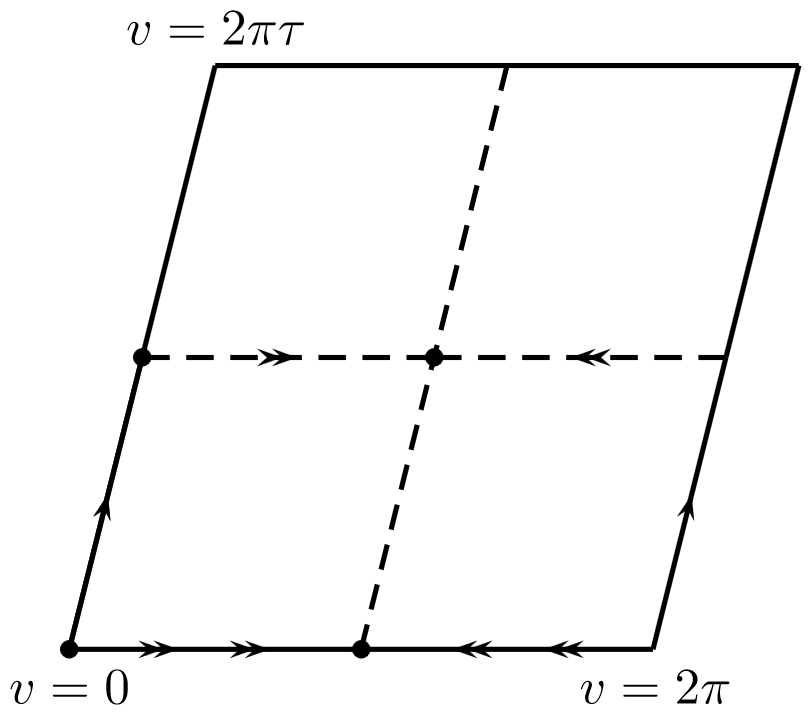
\includegraphics[width=0.85\textwidth]{figures/fig06.png}
  \caption{枕形几何是商 $T^2/\mathbb{Z}_2$。平面上的四点 $0,z,1,\infty$ 分别映到 $\mathbb{Z}_2$ 的不动点 $w=0,\pi,\pi(\tau+1),\pi\tau$。（原文 p.12，图 6）}
  \label{fig:6}
\end{figure}

% [Tutor Note: (3.25) 的 $q=e^{i\pi\tau}$ 是“半周期”nome：枕形的基本周期为 $2\pi$ 与 $2\pi\tau$，故 $q$ 的幂是 $e^{in\pi\tau}$。这与环面配分函数常用的 $q=e^{2\pi i\tau}$ 相差一个因子 2，是抄写 $\theta_3$ 级数时最常见的错误来源。]

从黎曼球上的坐标 $u$ 到枕形上的 $w$ 的显式映射为
\begin{equation}\label{eq:3-26}
  w=\frac{1}{(\theta_3(\tau))^2}\int_0^u\frac{dx}{\sqrt{x(1-x)(z-x)}},
\end{equation}
其中 $\theta_3(\tau)=\sum_{n=-\infty}^{\infty}q^{n^2}$ 是 Jacobi theta 函数之一。在枕形框架中，四个原初算符插入在四个角点 $w=0,\pi,\pi\tau,\pi(1+\tau)$，而共形块可以看作柱面上的传播子~\cite{r11}。

% 原文此处跨页（PDF 第 13 页末）："of as the propagator on the cylinder [11]"，
% 已在上一句收句；ch03b.tex 从 "Its matrix elements are written..." 续译。

